\chapter{Overview}

Now that we have introduced the problem,
we can flesh out our philosophy and overall
approach.

At a high level, there are three phases to
generating types:

\begin{enumerate}
  \item Instrumentation
  \item Runtime tracking
  \item Type reconstruction
\end{enumerate}

The first phase, \textbf{instrumentation}, involves
rewriting the code we wish to annotate such
that we can record its runtime behavior.
In this phase, we require the programmer to
indicate which code we wish to generate types
for, in advance.

Once instrumented, we observe our running program
via \textbf{runtime tracking}. To exercise our programs,
we usually run their unit tests, generative tests,
or just normally run the program (eg. to generate types for
a game, we can simply play the game for a few minutes).
We accumulate the results of tracking via \textbf{paths}.
If we think of types as trees and supply a label
for each branching path, our inference results
specify the type down a particular path in this tree.

Finally, the information collected during runtime tracking
is combined into annotations by our \textbf{inference algorithm}.
We first combine all inference result into a large tree of
types. If we were to convert this tree into annotations directly,
our annotations would be too specific---they would be too
deep and fine-grained.
Instead, our algorithm iterates over several passes to massage
this tree, generating good names for the nodes, compacting similar
types across the tree, and
eventually converting the tree into a directed graph by reconstructing
recursive types.

Let's demonstrate this pipeline, with our opening example.

...

\begin{verbatim}

\end{verbatim}

An important question to answer is ``how accurate are these annotations?''.
Unlike previous work in this area, we do not aim for soundness guarantees
in our generated types. 
Our main contribution is a tool that Clojure programmers
can use to help learn about and specify their programs.
In that spirit, annotations should meet several criteria.

\paragraph{Good names}
Typed Clojure and clojure.spec annotations are abundant
with useful names for types. A good name often increases
readability.
Good names can sometimes be reconstructed from the program source,
like function or parameter names, and other times 
we can use the shape of a type to summarize it.

\paragraph{Compact}
Idiomatic Clojure code rarely mixes certain types in the same position,
unless the program is polymorphic. Using this knowledge---which we observed
by the annotations and specs assigned to idiomatic Clojure 
code---we can rule out certain combinations of types to compact our
resulting output, without losing information that would help us
type check our programs.

\paragraph{Recursive}
Maps in Clojure are often heterogeneous, and recursively defined.
Typed Clojure and clojure.spec supplies mechanisms for the most
common case: maps of known keyword entries.
We strategically \textbf{squash} flat types to be recursive
based on their unrolled shape.
For example, a recursively defined union of maps almost always
contains a known keyword ``tag'' mapped to a keyword.
By identifying this tag, we can reconstruct a good recursive
approximation of this type.

\section{Naming}

For a type to be immediately useful to a programmer, it helps
to have a great name. We explored several avenues for
generating good names.

For types that occured as function arguments, the name of
the argument often indicated its role in the program.
Names like \textbf{config} or \textbf{env} are often used
for an environment being functionally threaded through
the program.

Similarly, types that occur as values in configuration
maps often have descriptive keys. In the Star Trek 
game, the configuration map maps \textbf{:stardate}
to a map that contains three number entries: 
\textbf{:start},
\textbf{:current}, and
\textbf{:end}.

What if a type occurs in the return position of a function?
Sometimes these are named by \textbf{let} binding the result
of the computation.

Failing these heuristics, we fall back of several approaches
to naming.
First, if we are naming a keyword map which is part of a tagged
union, we use the tag as the name. For example, if the tagged entry
maps \textbf{:op} to \textbf{:fn}, we name this map \textbf{FnOp}.
Failing that, for maps with less than three entries, we simply
enumerate its entries as the name.
Finally, for large keyword maps, we give an abbreviation
of its keyset as a name.

\begin{Verbatim}
(defn f [x] (inc x))
\end{Verbatim}

\begin{figure*}
\begin{Verbatim}
(defn vertices [m]
  (case (:op m)
    :leaf 1
    :node (+ 1 (:left m) (:right m))))
\end{Verbatim}
\label{code:vertices}
\end{figure*}

%%%% An old introductory example %%%%%%

%Consider the problem of inferring the type for
%the following Clojure program, a one
%argument function $f$ that increments numbers.
%
%\begin{verbatim}
%(defn f [x] (inc x))
%\end{verbatim}
%
%We might unit test this feature on the integers,
%to ensure incrementing $1$ gives $2$.
%
%\begin{verbatim}
%(deftest f-test
%  (is (= (f 1) 2)))
%\end{verbatim}
%
%We can instrument this program to observe its runtime behavior.
%
%\begin{verbatim}
%(deftest f-test
%  (is (= ((track f ['f]) 1) 2)))
%\end{verbatim}
%
%The $track$ function takes a value and a \emph{path},
%which tracks the subcomponent of the current environment
%the given value represents. For example, the path
%
%\begin{verbatim}
%  ['f :domain]
%\end{verbatim}
%
%represents the domain of $f$.
%
%After instrumentation we collect some inference results,
%associating paths with types: $path : \tau$.
%
%\begin{verbatim}
%  [['f :domain] Int]
%  [['f :range] Int]
%\end{verbatim}
%
%We combine this information into a type environment
%$\Gamma$ mapping variables to types: $\{x : \tau\}$.
%
%\begin{verbatim}
%  {x : [Int -> Int]}
%\end{verbatim}
%
%Now consider the case where we add a new unit test.
%
%\begin{verbatim}
%(deftest f-test
%  (is (= (f 1) 2))
%  (is (= (f 2.5) 3.5)))
%\end{verbatim}
%
%We now have a new set of inference results:
%
%\begin{verbatim}
%  [['f :domain] Num]
%  [['f :range] Num]
%\end{verbatim}
%
%which we want to combine with our previously inferred type environment
%
%\begin{verbatim}
%  {x : [Int -> Int]}
%\end{verbatim}
%
%How do join $[Int -> Int]$
%and $[Num -> Num]$?
%We have several options.
%
%
%\begin{verbatim}
%[(I Num Int) -> (U Num Int)]
%\end{verbatim}
%
%\begin{verbatim}
%[(U Num Int) -> (U Num Int)]
%\end{verbatim}
%
%\begin{verbatim}
%(IFn [Int -> Int]
%     [Num -> Num])
%\end{verbatim}

\begin{figure}
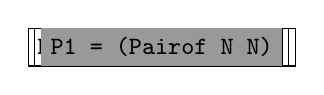
\begin{tikzpicture}[level distance=0.8cm, scale=0.9]
\tikzstyle{every node}=[font=\small]
\tikzset{grow'=down}
\tikzset{every tree node/.style={align=center,anchor=north}}
\Tree [.\node[draw](P0){\texttt{P0 = (Pairof P1 P2)}};
        [.\node[draw](P2){\texttt{P2 = (Pairof P3 N)}};
          [ \texttt{N} ]
          [.\node[draw](P3){\texttt{P3 = (Pairof N N)}};
            [ \texttt{N} ] [ \texttt{N} ]]
]
        [.\node[fill=gray!80](P1){\texttt{P1 = (Pairof N N)}};
          [ \texttt{N} ] [ \texttt{N} ] ]
 ]
\end{tikzpicture}
%
%\hspace{0.15cm}
%
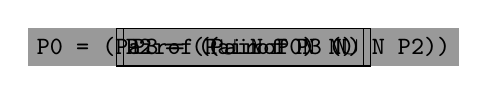
\begin{tikzpicture}[level distance=0.8cm]
\tikzstyle{every node}=[font=\small]
\tikzset{grow'=down}
\tikzset{every tree node/.style={align=center,anchor=north}}
\Tree [.\node[fill=gray!80](P0){\texttt{P0 = (Pairof ($\cup$ N P0) ($\cup$ N P2))}};
        [.\node[draw](P2){\texttt{P2 = (Pairof P3 N)}};
          [ \texttt{N} ]
          [.\node[draw]{\texttt{P3 = (Pairof N N)}};
            [ \texttt{N} ] [ \texttt{N} ]]
]
          [ \texttt{N} ] [ \texttt{N} ] 
 ]
%\draw[semithick,->] (P1)..controls +(west:1) and +(west:1)..(P0);
\end{tikzpicture}
\end{figure}

